\documentclass[12pt]{article}

\usepackage{sbc-template}
\usepackage[hidelinks]{hyperref}
\usepackage{graphicx,url}
\usepackage{xcolor}

\usepackage[brazil]{babel}   
%\usepackage[latin1]{inputenc}  
\usepackage[utf8]{inputenc}
     
\sloppy

\title{\textbf{Microcontrolador Arduino UNO}}

\author{Raul Ramires\inst{1}}


\address{Departamento de Informática -- Universidade Estadual de Maringá
	(UEM)\\
	Maringá -- PR -- Brazil
	\email{ra82293@uem.br}
}

\begin{document} 

\maketitle

\section{Introdução}
	O arduino é uma placa microcontroladora baseada no microcontrolador ATMega e pode ser integrada com uma grande diversidade de componentes e sensores. O projeto a ser desenvolvido propõe a configuração do ambiente de trabalho e a realização de diversos experimentos com diferentes sensores.

\section{Ambiente de Trabalho}
	O arduino possui uma IDE \textit{Integrated Development Environment} chamada de ``Arduino IDE'', que é onde serão escritos os códigos para que depois sejam enviados ao arduino e executado.

\subsection{Download da IDE}
	Para fazer o download da IDE basta ir ao \href{https://www.arduino.cc/en/Main/Software}{\underline{\textcolor{blue}{site do arduino}}} e escolher a versão de acordo com o sistema operacional utilizado, estando disponível para Windows, Linux e MacOS.

\section{Programação}
	A programação do arduino é feita na linguagem C++ e possui uma grande quantidade de bibliotecas prontas para a utilização de sensores.

\subsection{Estrutura do código}
	A Figura \ref{figEstruturaCodigo} mostra a estrutura básica de um código para arduino. Esse código é dividido em duas funções: a função \textit{setup} e a função \textit{loop}.

	\begin{figure}[h!]
		\centering
		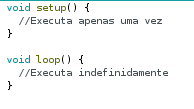
\includegraphics[scale=1.3]{Imagens/figEstrutura.png}
		\caption{Estrutura do código.}
		\label{figEstruturaCodigo}
	\end{figure}

	A função \textit{setup} será executada apenas uma vez no início do programa, geralmente é aqui que ficam as definições de pinos de entradas e saídas e algumas variáveis globais.
	A função \textit{loop} será executada infinitamente enquanto o arduino estiver ligado, é aqui que serão feitas as leituras de sensores e decisões de ações com bases nos dados lidos dos sensores.

\subsection{Upload do código}
	Para realizar o \textit{upload} do código para a placa do arduino, basta clicar no botão ``carregar'', então o código será compilado e carregado para o arduino e então começar a execução.

\section{Experimentos}
	Nessa seção serão realizados vários experimentos com o arduino, utilizando uma grande diversidade de componentes e sensores.

	Todos os experimentos realizados nesse trabalho estão disponíveis no repositório no \href{https://github.com/ramires352/Arduino-UEM}{\underline{\textcolor{blue}{\textit{GitHub}}}} e os esquemáticos dos circuitos estão disponíveis no \href{https://www.tinkercad.com/users/8OFhdueEmAr-rrramires?category=circuits&sort=likes&view_mode=default}{\underline{\textcolor{blue}{\textit{Tinkercad}}}}.

\subsection{Piscar um LED}
	Para realizar esse experimentos será necessário um LED, uma \textit{protoboard} e dois \textit{jumpers}.

	A \textit{protoboard} é construída como uma matriz, onde cada coluna possui 5 pontos de contato que são interligados entre si, porém uma coluna é isolada de sua vizinha, sendo necessário a utilização de um \textit{jumper} para interligar duas colunas.

	Alguns modelos de \textit{protoboard} possuem dois barramentos laterais, um negativo e um positivo que percorrem a \textit{protoboard} inteira. O padrão de utilização desses barramentos é ligar o 5V no barramento vermelho e o GND no barramento preto, ficando assim mais simples de realizar a alimentação dos componentes utilizados.

	A Figura \ref{figProtoboard} mostra o esquema de uma \textit{protoboard} de 360 pontos.

	\begin{figure}[h!]
		\centering
		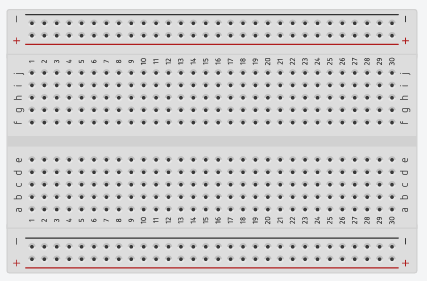
\includegraphics[scale=0.5]{Imagens/figProtoboard.png}
		\caption{\textit{Protoboard} de 360 pontos}
		\label{figProtoboard}
	\end{figure}

	A Figura \ref{figExp1PiscarLEDesq} mostra o esquema do circuito para piscar um LED, utilizando o arduino.

	\begin{figure}[h!]
		\centering
		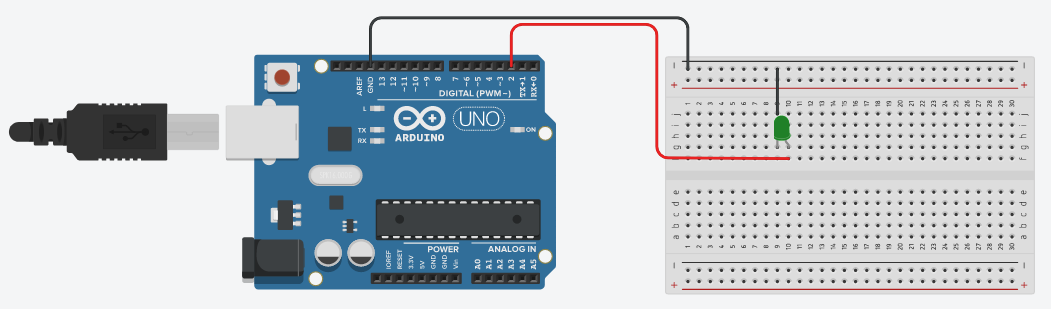
\includegraphics[scale=0.3]{Imagens/Experimentos/1-PiscarLED/1-PiscarLED.png}
		\caption{Esquemático do circuito do experimento 1.}
		\label{figExp1PiscarLEDesq}
	\end{figure}

	Nesse circuito o pino digital 2 do arduino está ligado na coluna 10 da protoboard, onde, nessa mesma coluna está ligado o terminal positivo do LED. O terminal negativo do LED está ligado na coluna 9, que possui um \textit{jumper} para o barramento preto, que por sua vez está ligado ao GND do arduino. Sendo assim o LED irá acender quando o arduino enviar o sinal de 5V no pino 2.

	A Figura \ref{figExp1PiscarLEDcod} mostra o código que fará com que o arduino pisque o LED.

	\begin{figure}[h!]
		\centering
		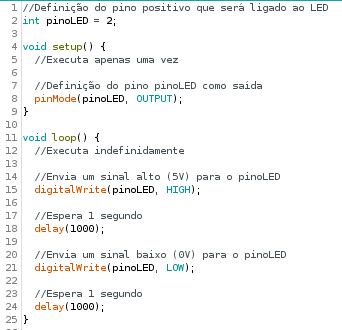
\includegraphics[scale=0.8]{Imagens/Experimentos/1-PiscarLED/1-PiscarLEDcod.png}
		\caption{Código do experimento 1.}
		\label{figExp1PiscarLEDcod}
	\end{figure}

\subsection{Mudar o brilho de um LED}
	Para realizar esse experimento será necessário um LED, um potenciômetro e um resistor de 220$\Omega$.

	O potenciômetro é um resistor capaz de variar sua resistencia, para esse experimento, o arduino irá ler esse valor de resistência e associar a um valor de tensão e enviar ao LED, variando assim o brilho do LED. Como esse valor é variável, é necessário conectar o potenciômetro a uma porta analógica do arduino.

	A Figura \ref{figExp2BrilhoLEDesq} mostra o esquemático do circuito do experimento.

	\begin{figure}[h!]
		\centering
		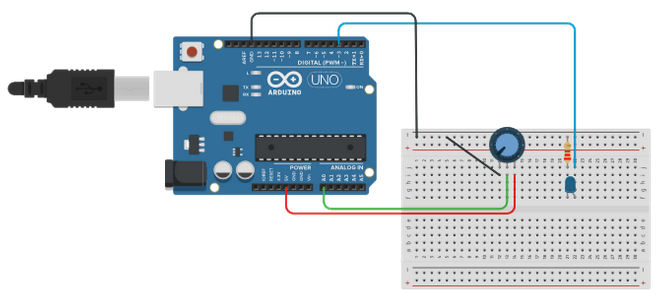
\includegraphics[scale=0.4]{Imagens/Experimentos/2-brilhoLED/2-brilhoLEDesq.png}
		\caption{Esquemático do circuito do experimento 2.}
		\label{figExp2BrilhoLEDesq}
	\end{figure}

	O arduino faz a leitura do potenciômetro em um valor de 0 a 1023. Para usar esse valor para acender o LED, é necessário fazer uma conversão para um valor de 0 a 255. Para isso é utilizado a função \textit{map}, que é responsável por fazer esse mapeamento de um intervalo para outro.

	A figura \ref{figExp2BrilhoLEDcod} mostra o código do experimento 2.\\

	\begin{figure}[h!]
		\centering
		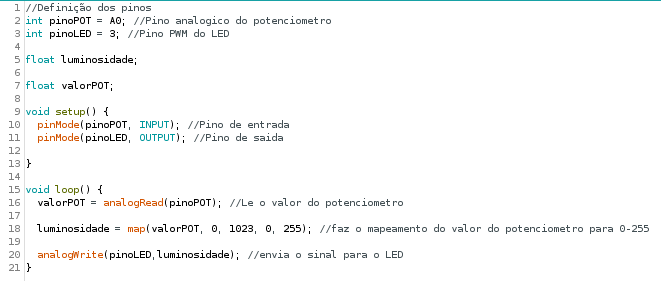
\includegraphics[scale=0.6]{Imagens/Experimentos/2-brilhoLED/2-brilhoLEDcod.png}
		\caption{Código do experimento 2.}
		\label{figExp2BrilhoLEDcod}
	\end{figure}

\subsection{Sensor de luz}
	Esse experimento tem como objetivo controlar uma barra de LEDs a partir de um LDR (\textit{Light Dependent Resistor}). O LDR é um resistor que varia sua resistência de acordo com a luz que incide sobre ele, quanto maior a quantidade de luz, menor a resistência do LDR. Como o LDR é um componente que possui um valor de resistência variável, é necessário conectá-lo a uma porta analógica do arduino.

	Para esse experimento, quanto maior a luz incidente sobre o LDR, menos LEDs irão acender.

	A Figura \ref{figExp3LDResq} mostra o esquemático do circuito do experimento 3.

	\begin{figure}[h!]
		\centering
		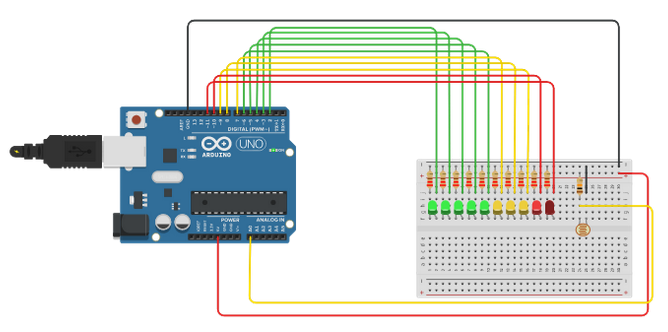
\includegraphics[scale=0.4]{Imagens/Experimentos/3-LDR-LEDGraph/3-LDR-LEDGraphEsq.png}
		\caption{Esquemático do circuito do experimento 3.}
		\label{figExp3LDResq}
	\end{figure}

	A Figura \ref{codigoExp3} mostra o código do experimento 3.

	\begin{figure}[h!]
		\centering
		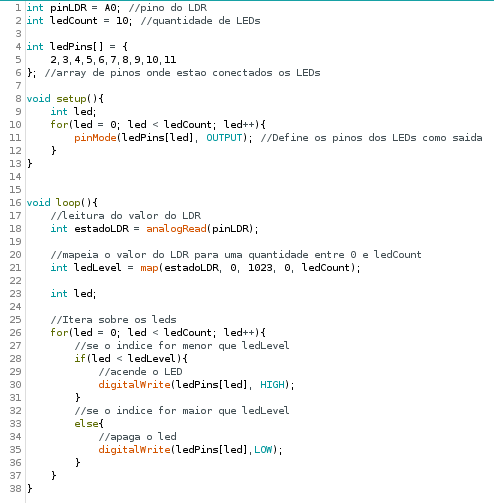
\includegraphics[scale=0.39]{Imagens/Experimentos/3-LDR-LEDGraph/codigo.png}
		\caption{Código do experimento 3.}
		\label{codigoExp3}
	\end{figure}

\subsection{Display de 7 Segmentos}
	Esse experimento faz o controle de um display de 7 segmentos utilizando um botão para exibir os dígitos de 0 a 9. O display incia exibindo o dígito 0 e incrementa um dígito quando o botão é pressionado. Os segmentos do display são nomeados de acordo com a Figura \ref{figSegmentosDisplay} \cite{siteDisplay7}.

	\begin{figure}[h!]
		\centering
		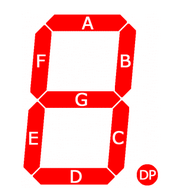
\includegraphics[scale=0.5]{Imagens/Experimentos/4-Display7Seg/7segmentos.png}
		\caption{Segmentos do display.}
		\label{figSegmentosDisplay}
	\end{figure}

	Para acender um segmento o arduino deve enviar um sinal alto para o segmento, e para apagar deve enviar um sinal baixo.

	A Figura \ref{figPinosDisplay} mostra a pinagem do display. Para esse experimento não será utilizado o ponto decimal.

	\begin{figure}[h!]
		\centering
		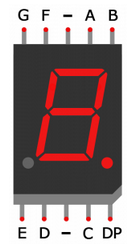
\includegraphics[scale=0.5]{Imagens/Experimentos/4-Display7Seg/pinosDisplay.png}
		\caption{Pinagem do display de 7 segmentos.}
		\label{figPinosDisplay}
	\end{figure}

	O botão é definido como \textit{INPUT\_PULLUP} para utilizar um resistor interno do arduino e simplificar o circuito, por conta disso, o arduino interpreta o botão como estado alto quando não pressionado e estado baixo quando pressionado. Para detectar o acionamento do botão é necessário considerar o estado atual do botão e o estado anterior, pois o arduino faz a leitura do botão um grande número de vezes por segundo, sendo assim é necessário esse tratamento para evitar que o arduino interprete que o botão foi acionado diversas vezes em apenas um acionamento.

	A Figura \ref{figExp4botao} mostra o trecho de código que faz a leitura do botão.

	\begin{figure}[h!]
		\centering
		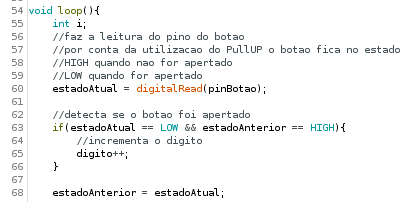
\includegraphics[scale=0.65]{Imagens/Experimentos/4-Display7Seg/codigoBotao.png}
		\caption{Código que detecta o acionamento do botão.}
		\label{figExp4botao}
	\end{figure}

\bibliographystyle{sbc}
\bibliography{referencias}

\end{document}
